\documentclass{article}
\usepackage[utf8]{inputenc}
\usepackage[spanish]{babel}
\usepackage{listings}
\usepackage{graphicx}
\graphicspath{ {images/} }
\usepackage{cite}

\begin{document}

\begin{titlepage}
    \begin{center}
        \vspace*{1cm}
            
        \Huge
        \textbf{Parcial II 2021-1 Informática 2}
            
        \vspace{0.5cm}
        \LARGE
        Informe de Implementación de la Solución del Desafío
            
        \vspace{1.5cm}
            
        \textbf{Juan Diego Cabrera Moncada}\\
            
        \vfill
            
        \vspace{0.8cm}
            
        \Large
        Despartamento de Ingeniería Electrónica y Telecomunicaciones\\
        Universidad de Antioquia\\
        Medellín\\
        Septiembre de 2021
            
    \end{center}
\end{titlepage}

\tableofcontents
\newpage
\section{Clases implementadas}
\section{Esquema de la estructura final de las clases implementadas}
\section{Módulos de código implementado donde interactúan las diferentes clases}
\section{Estructura del circuito montado}
En caso de modificaciones, el último montaje de la matriz de Neopixeles es la versión final del proyecto en Tinkercad. La primera versión corresponde a una matriz de Neopixeles de 8 x 8 en la cual se usa el pin digital 2 del Arduino Uno como pin de salida para transmitir la información leída del archivo de texto y guardada en un arreglo tridimensional de valores enteros, usando los métodos de la librería correspondiente de dichos componentes para su efectiva configuración a partir del uso del pin 2 del Arduino Uno. En esta matriz, a pesar de estas dispuestos como tiras de 8 neopixeles una encima de la otra, en cuanto a conexiones, están conectados de modo que la entrada de la tira de la fila superior está conectada en su puerto de entrada al pin 2 y su puerto negativo y positivo a los que le corresponden al arduino, haciendo uso a su vez de un suministro de energía para asegurar la transmisión de suficiente voltaje para las 8 tiras en el circuito. Los segundos puertos de positivo, negativo y el puerto de salida están conectados, respectivamente, a los puertos positivo, negativo y de entrada de la tira de 8 neopixeles de la fila inferior a ella. Y así sucesivamente hasta llegar a la tira de neopixeles de la última fila, cuyo puerto de salida, uno de los positivos y uno de los negativos se encuentra desconectado pues corresponde a la última fila. En primera instancia, se espera que, en dado caso que se modifique el circuito, no implique un cambio en las conexiones del circuito drásticamente, sino únicamente en la cantidad de neopixeles que se desea usar por fila y/o columna.
\begin{figure} 
    \centering
    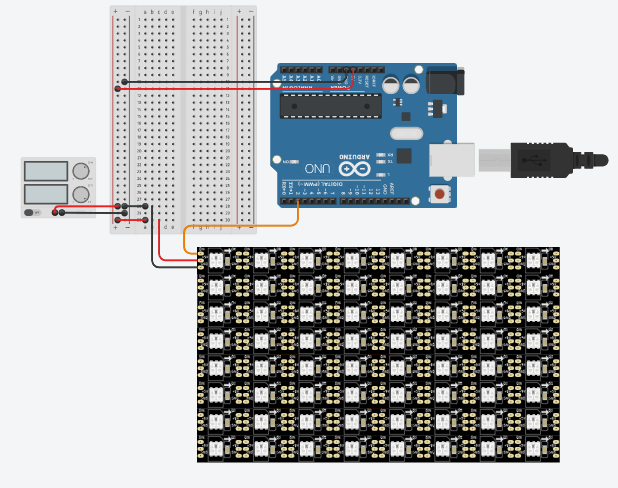
\includegraphics[width=10cm]{matriz8x8Neopixeles.png}
    \caption{Matriz de 8 x 8 Neopixeles}
    \label{fig:mat8x8_neo}
\end{figure}
\section{Problemas presentados durante la implementación}
Al realizar pruebas con código en el proyecto en Tinkercad, en primer lugar, hubo una serie de problemas al usar un buffer de un tamaño lo suficientemente grande para que el usuario ingresase línea por línea el contenido del archivo de texto de tal modo que cada línea representara una de las filas de la matriz, con el fin de que el usuario tenga que hacer el menor esfuerzo posible, no fue viable debido a que al usar tanto memoria en Stack como por memoria dinámica, el buffer solo alcanzaba a captar un poco más de la mitad de la línea que se ingresaba por medio del monitor en serie, por lo cual decidí que tocaba hacer que cada línea representara la información de los 3 colores de 4 neopixeles de una misma fila, de modo que por cada 2 ingresos de datos, se cambia el número de la fila. Dicha información ingresada por el usuario es almacenada en una matriz tridimensional de enteros llamada "pixeles", la cual va a ser indexada con el objetivo de configurar los neopixeles con el método "setPixelColor" que proporciona la librería de Adafruit Neopixel. De esta forma, se configuró todo dentro de una función, además de organizar dentro de una función las instrucciones que se le dan al usuario una vez termina de representar su bandera así como cuando inicializa el programa. De la misma forma, se creó una función para que el usuario tenga la opción de verificar el correcto funcionamiento de los neopixeles de la matriz de 8 x 8. A continuación, la primera versión organizada del código en Tinkercad descrito anteriormente:
\begin{lstlisting}[language=C++, label=prueba_ingresotxtymanualgeneraltink]
#include <Adafruit_NeoPixel.h>

#define LED_PIN 2

#define LED_COUNT 64

Adafruit_NeoPixel leds(LED_COUNT, LED_PIN, NEO_GRB + NEO_KHZ800);

void verificacion();
void ingreso_info();
void main_instruc();

void setup()
{
  leds.begin();
  Serial.begin(9600);
  int pixeles[3][LED_COUNT/8][LED_COUNT/8] = {0};
  main_instruc();
}

void loop()
{
  if(Serial.available()>0){
    int numero = Serial.parseInt();
    if(numero == 1){
      verificacion();
    }
    else if(numero == 2){
      Serial.println("Por favor, ingrese en el monitor en serie el contenido del archivo");
      Serial.println("de texto dado en el primer programa usado ingresando linea por linea,");
      Serial.println("(Es decir el archivo de texto que se le menciono mantener abierto para este segundo programa");
      Serial.println("exactamente como se encuentra escrito. No modifique nada del contenido.");
      Serial.println("En el monitor en serie, se le va a mostrar un aviso para poder copiar 1 linea");
      Serial.println("y pegarla en el recuadro del monitor en serie, en su parte inferior, habilitado para pegar dicha linea.");
      Serial.println("Una vez verifique que la linea ha sido copiada y pegada correctamente, oprima enter para ingresarla.");
      Serial.write("\n\n\n");
      ingreso_info();
      main_instruc();
    }
    else{
      Serial.println("El numero ingresado no se encuentra entre las opciones dadas.");
      Serial.println("Por favor, ingrese otro numero.");
      main_instruc();
    }
  }
}

void main_instruc(){
  Serial.println("Estimado cliente, para hacer uso de esta matriz de neopixeles,");
  Serial.println("por favor, en el monitor en serie, escriba:");
  Serial.println("1 para verificar el correcto funcionamiento de la matriz");
  Serial.println("2 para representar en la matriz la imagen de la bandera escogida en el anterior programa");
}

void verificacion(){
  Serial.println("Verificacion de Matriz de Neopixeles 8 x 8");
  for(int i = 0; i < LED_COUNT; i += 1){
    leds.setPixelColor(i, 207, 97, 62);
  }
  leds.show();
  delay(3000);
  Serial.println("Finalizando Verificacion...");
  for(int i = 0; i < LED_COUNT; i += 1){
    leds.setPixelColor(i, 0, 0, 0);
  }
  leds.show();
}

void ingreso_info(){
  int *ptr_cont= NULL;
  ptr_cont = new int;
  *ptr_cont = 0;
  int num_color = 0, f = 0, c = 0;
  while(*ptr_cont <= 15){
    delay(1000);
    if(Serial.available()>0){
      const int length = 48;
      char *fil = new char[length];
      int user = Serial.readBytes(fil,length);
      int valColor[3] = {0};
      for(int i = 0; i<=length-1; i++){
        Serial.println(int(fil[i]));
        if(int(fil[i]) == 44){ // ,
          num_color++;
          int col = 0;
          for(int i = 2; i>=0; i--){
            int mult = 1;
            if(valColor[i] != 46){ // No hay mas .
              col = col + (valColor[i]-48)*mult;
              mult = mult*10;
            }
            pixeles[num_color][f][c] = col; //Asignacion color
          }
          
        }
        else if(int(fil[i]) == 59){ // ;
          for(int i = 0; i<=2;i++) valColor[i] = 0;
          num_color = 0;
          c++;
        }
      }
      delete[] fil;
      if(*ptr_cont%2!=0){
        f++;
        c=0;
      }
      *ptr_cont = *ptr_cont + 1;
    }
  }
  delete [] ptr_cont;
}
\end{lstlisting}
Dicho código tenía unos fallos en cuanto al uso de memoria e indexaciones hechas de manera errónea, por lo cual se hizo una serie de modificaciones para mejorar este aspecto, no obstante aún se mantiene un problema de guardado de cantidades enteras erróneas y, en adición a esto, parte del código se está ejecutando más veces de las que se tiene previsto, haciendo que la cantidad de colores que se va a guardar para cada pixel sea de 5 en vez de 3.
\begin{lstlisting}[language=C++, label=error_guardarints]
#include <Adafruit_NeoPixel.h>

#define LED_PIN 2

#define LED_COUNT 64

Adafruit_NeoPixel leds(LED_COUNT, LED_PIN, NEO_GRB + NEO_KHZ800);

void verificacion();
void ingreso_info();
void main_instruc();

int pixeles[3][LED_COUNT/8][LED_COUNT/8] = {0};

void setup()
{
  leds.begin();
  Serial.begin(9600);
  main_instruc();
}

void loop()
{
  if(Serial.available()>0){
    int numero = Serial.parseInt();
    if(numero == 1){
      verificacion();
    }
    else if(numero == 2){
      Serial.println("Por favor, ingrese en el monitor en serie el contenido del archivo");
      Serial.println("de texto dado en el primer programa usado ingresando linea por linea,");
      Serial.println("(Es decir el archivo de texto que se le menciono mantener abierto para este segundo programa");
      Serial.println("exactamente como se encuentra escrito. No modifique nada del contenido.");
      Serial.println("En el monitor en serie, se le va a mostrar un aviso para poder copiar 1 linea");
      Serial.println("y pegarla en el recuadro del monitor en serie, en su parte inferior, habilitado para pegar dicha linea.");
      Serial.println("Una vez verifique que la linea ha sido copiada y pegada correctamente, oprima enter para ingresarla.");
      Serial.write("\n\n\nIngrese la primera linea.");
      ingreso_info();
      main_instruc();
    }
    else{
      Serial.println("El numero ingresado no se encuentra entre las opciones dadas.");
      Serial.println("Por favor, ingrese otro numero.");
      main_instruc();
    }
  }
}

void main_instruc(){
  Serial.println("Estimado cliente, para hacer uso de esta matriz de neopixeles,");
  Serial.println("por favor, en el monitor en serie, escriba:");
  Serial.println("1 para verificar el correcto funcionamiento de la matriz");
  Serial.println("2 para representar en la matriz la imagen de la bandera escogida en el anterior programa");
}

void verificacion(){
  Serial.println("Verificacion de Matriz de Neopixeles 8 x 8");
  for(int i = 0; i < LED_COUNT; i += 1){
    leds.setPixelColor(i, 207, 97, 62);
  }
  leds.show();
  delay(3000);
  Serial.println("Finalizando Verificacion...");
  for(int i = 0; i < LED_COUNT; i += 1){
    leds.setPixelColor(i, 0, 0, 0);
  }
  leds.show();
}

void ingreso_info(){
  int *ptr_cont= NULL, *num_color = NULL, *f = NULL, *c = NULL;
  ptr_cont = new int, num_color = new int, f = new int, c = new int;
  *ptr_cont = 0, *num_color = 0, *f = 0, *c = 0;
  while(*ptr_cont <= 15){
  	delay(500);
    if(Serial.available()>0){
    	const int length = 48;
    	char *fil = new char[length];
      	int user = Serial.readBytes(fil,length);
      	int valColor[3] = {0};
      	for(int i = 0; i<=length-1; i++){
        	if(int(fil[i]) == 44){ // ,
          		int col = 0, mult = 1;
          		for(int i = 2; i >=0; i--){
            		if(valColor[i] != 46){ // No hay mas .
              			col = col + (valColor[i]-48)*mult;
              			mult = mult*10;
            		}
                }
              	Serial.print(*num_color);
                Serial.print(",");
                Serial.print(*f);
                Serial.print(",");
                Serial.print(*c);
                Serial.print("=");
                Serial.println(col);
              	pixeles[*num_color][*f][*c] = col; //Asignacion color
                for(int i = 0; i<=2;i++){
                	valColor[i] = 0;
              	}
              	*num_color= 1+*num_color;
    	    }
        	else if(int(fil[i]) == 59){ // ;
              	int col = 0, mult = 1;
          		for(int i = 2; i >=0; i--){
            		if(valColor[i] != 46){ // No hay mas .
              			col = col + (valColor[i]-48)*mult;
              			mult = mult*10;
            		}
                Serial.print(*num_color);
                Serial.print(",");
                Serial.print(*f);
                Serial.print(",");
                Serial.print(*c);
                Serial.print("=");
                Serial.println(col);
            	pixeles[*num_color][*f][*c] = col; //Asignacion color
                *num_color = 10+*num_color;
                }
              	for(int i = 0; i<=2;i++){
                	valColor[i] = 0;
              	}
          		*num_color = 0;
          		*c = 1 + *c;
        	}
            else{
            	valColor[i%4] = int(fil[i]);
            }
      	}
      	for(int i = 0; i<=length-1; i++){
        	//Serial.println(int(fil[i]));
        }
      	if(*ptr_cont!=15){
        	Serial.println("Ingrese la siguiente linea.");
      	}
      	if(*ptr_cont%2!=0){
          		*f = 1 + *f;
          		*c=0;
       	}
      	delete[] fil;
	    *ptr_cont = *ptr_cont + 1;
    }
  }
  delete [] ptr_cont, num_color, f, c;
}
\end{lstlisting}
Una vez resuelto dicho problema, se procedió a la creación de la función representar(), la cual se encarga de la representación de los valores enteros extraídos del archivo de texto, ahora guardados en el arreglo tridimensional de enteros "pixeles". No obstante, surgió un nuevo problema con la función verificación, pues, a pesar de no tener modificaciones en ningún aspecto, se comenzó a presentar fallas en la representación del color asignado para mostrar en todos los neopixeles de la matriz, esto hecho con el objetivo de que esto mostrase que, efectivamente, es funcional. De la misma forma, este problema se presentó cuando se trató de configurar los neopixeles de la matriz dentro de la función representar(). A pesar de ello, se pudo confirmar que tanto el guardado de la información como la indexación de los valores del arreglo "pixeles" fueron exitosos, por lo cual este sería el último problema aparente por resolver en cuanto a la parte de Tinkercad:
\begin{lstlisting}[language=C++, label=error_electronica]
#include <Adafruit_NeoPixel.h>

#define LED_PIN 2

#define LED_COUNT 64

Adafruit_NeoPixel leds(LED_COUNT, LED_PIN, NEO_GRB + NEO_KHZ800);

void verificacion();
void ingreso_info();
void representar();
void main_instruc();

int pixeles[3][LED_COUNT/8][LED_COUNT/8] = {0};

void setup()
{
  leds.begin();
  Serial.begin(9600);
  main_instruc();
}

void loop()
{
  if(Serial.available()>0){
    int numero = Serial.parseInt();
    if(numero == 1){
      verificacion();
    }
    else if(numero == 2){
      Serial.println("Por favor, ingrese en el monitor en serie el contenido del archivo");
      Serial.println("de texto dado en el primer programa usado ingresando linea por linea,");
      Serial.println("(Es decir el archivo de texto que se le menciono mantener abierto para este segundo programa");
      Serial.println("exactamente como se encuentra escrito. No modifique nada del contenido.");
      Serial.println("En el monitor en serie, se le va a mostrar un aviso para poder copiar 1 linea");
      Serial.println("y pegarla en el recuadro del monitor en serie, en su parte inferior, habilitado para pegar dicha linea.");
      Serial.println("Una vez verifique que la linea ha sido copiada y pegada correctamente, oprima enter para ingresarla.");
      Serial.write("\n\n\nIngrese la primera linea.");
      ingreso_info();
      representar();
      main_instruc();
    }
    else{
      Serial.println("El numero ingresado no se encuentra entre las opciones dadas.");
      Serial.println("Por favor, ingrese otro numero.");
      main_instruc();
    }
  }
}

void main_instruc(){
  Serial.println("Estimado cliente, para hacer uso de esta matriz de neopixeles,");
  Serial.println("por favor, en el monitor en serie, escriba:");
  Serial.println("1 para verificar el correcto funcionamiento de la matriz");
  Serial.println("2 para representar en la matriz la imagen de la bandera escogida en el anterior programa");
}

void verificacion(){
  Serial.println("Verificacion de Matriz de Neopixeles 8 x 8");
  for(int i = 0; i < LED_COUNT; i += 1){
    leds.setPixelColor(i, 207, 97, 62);
  }
  leds.show();
  delay(3000);
  Serial.println("Finalizando Verificacion...");
  for(int i = 0; i < LED_COUNT; i += 1){
    leds.setPixelColor(i, 0, 0, 0);
  }
  leds.show();
}

void ingreso_info(){
  int *ptr_cont= NULL, *num_color = NULL, *f = NULL, *c = NULL;
  ptr_cont = new int, num_color = new int, f = new int, c = new int;
  *ptr_cont = 0, *num_color = 0, *f = 0, *c = 0;
  while(*ptr_cont <= 15){
  	delay(500);
    if(Serial.available()>0){
    	const int length = 48;
    	char *fil = new char[length];
      	int user = Serial.readBytes(fil,length);
      	int valColor[3] = {0};
      	for(int i = 0; i<=length-1; i++){
        	if(int(fil[i]) == 44){ // ,
          		int col = 0, mult = 1;
          		for(int i = 2; i >=0; i--){
            		if(valColor[i] != 46){ // No hay mas .
              			col = col + (valColor[i]-48)*mult;
              			mult = mult*10;
            		}
                }
              	/*Serial.print(*num_color);
                Serial.print(",");
                Serial.print(*f);
                Serial.print(",");
                Serial.print(*c);
                Serial.print("=");
                Serial.println(col);*/
              	pixeles[*num_color][*f][*c] = col; //Asignacion color
              	*num_color= 1+*num_color;
    	    }
        	else if(int(fil[i]) == 59){ // ;
              	int col = 0, mult = 1;
          		for(int i = 2; i >=0; i--){
            		if(valColor[i] != 46){ // No hay mas .
              			col = col + (valColor[i]-48)*mult;
              			mult = mult*10;
            		}
                }
                /*Serial.print(*num_color);
                Serial.print(",");
                Serial.print(*f);
                Serial.print(",");
                Serial.print(*c);
                Serial.print("=");
                Serial.println(col);*/
            	pixeles[*num_color][*f][*c] = col; //Asignacion color
          		*num_color = 0;
          		*c = 1 + *c;
        	}
            else{
            	valColor[i%4] = int(fil[i]);
            }
      	}
      	if(*ptr_cont!=15){
        	Serial.println("Ingrese la siguiente linea.");
      	}
      	if(*ptr_cont%2!=0){
          		*f = 1 + *f;
          		*c=0;
       	}
      	delete[] fil;
	    *ptr_cont = *ptr_cont + 1;
    }
  }
  delete [] ptr_cont, num_color, f, c;
}
void representar(){
  	int *neo_indx = new int;
    for(int fil = 0; fil < LED_COUNT/8; fil++){
       	for(int col = 0; col < LED_COUNT/8; col++){
            leds.setPixelColor(*neo_indx,pixeles[0][fil][col],pixeles[1][fil][col],pixeles[2][fil][col]);
          	int red = pixeles[0][fil][col];
          	int green = pixeles[1][fil][col];
          	int blue = pixeles[2][fil][col];
          	Serial.println(red);
        	Serial.println(green);
         	Serial.println(blue);
          	Serial.println();
        	*neo_indx = *neo_indx + 1;
        }
      	*neo_indx = *neo_indx + 1;
    }
  	leds.show();
  	delete [] neo_indx;
}
\end{lstlisting}
\bibliographystyle{IEEEtran}
\bibliography{references}

\end{document}